\documentclass{ctexart}
\usepackage{graphicx}
\usepackage{caption}
\usepackage{float}
\usepackage{amsmath}
\usepackage{fancyhdr}
\usepackage{xunicode-addon}
\usepackage{booktabs}
\usepackage[a4paper,hmargin=1.25in,vmargin=1in]{geometry}
% !TeX program = xelatex
\title{\begin{figure}[H]
	\centering 
	\includegraphics[height=7cm,width=14cm]{E:/Pictures/中科大.jpg}
	\end{figure}\Huge\textbf{Lab 4}\\\huge{乳腺癌数据集分析}}
\date{}
\punctstyle{banjiao} 
\pagestyle{fancy}
	\fancyhead[C]{\LARGE\textbf{Report 4}}
	\fancyhead[L]{}
	\fancyhead[R]{}
	\fancyfoot[C]{\thepage}
\begin{document}
	\maketitle
	\thispagestyle{empty}
	
	\[\makebox{\Large{姓名:\underline{\makebox[5cm]{高茂航}}}}\]
	
    \[\makebox{\Large{学号:\underline{\makebox[5cm]{PB22061161}}}}\]
	
	$$\makebox{\Large{日期:\underline{\makebox[5cm]{2024.5.16}}}}$$
	
	\clearpage

	\pagenumbering{arabic}
    \section{Task1}
    \subsection{Algorithm Description}
	
	使用$df.isnull().sum()$判断有缺失项的列,使用$df.dropna()$删除有缺失项的行,使用$df.value\_counts()$显示一列中的数据分布,快速找出异常项后用$df.replace()$替换为正常值,
	等函数对数据集进行处理。
	
	对于Q3,遍历excel文件每行的Description列的所有元素放到一个列表中,
	以把df的值替换为索引,但是处理时发现deg-malig是整数类型而非字符串,因此一开始报错了,后来将这列转为字符串类型后就可以了。
	此外,还碰到一个问题是node-caps和irradiat这两列的值都是yes/no,一开始在替换时会把node-caps的索引赋给irradiat,
	因此在替换到irradiat时要特别找到第二个yes/no的索引。

\subsection{Results}
\subsubsection{Q1}
\begin{figure}[H]
	\centering 
	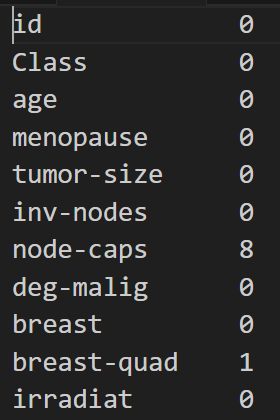
\includegraphics[height=5cm,width=3cm]{1.png}
	\end{figure}
	从结果可看出只有node-caps列和breast-quad列有缺失项,因此删除了这两行。
	\subsubsection{Q2}
	\begin{figure}[H]
		\centering 
		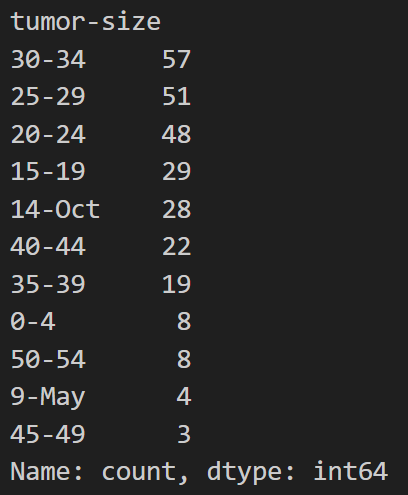
\includegraphics[height=7cm,width=6cm]{2.png}
		\end{figure}
		可看出tumor-size列有异常值'14-Oct'、'9-May',需要将其替换为正常值。
		\begin{figure}[H]
			\centering 
			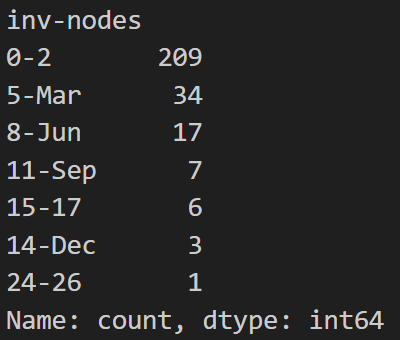
\includegraphics[height=6cm,width=6cm]{3.png}
			\end{figure}
可看出inv-nodes列有异常值'5-Mar'、'8-Jun'、'11-Sep'、'14-Dec',需要将其替换为正常值。	
			\subsubsection{Q3}
		$\{0: 'Class=no-recurrence-events', 1: 'Class=recurrence-events', 2: 'age=10-19', 3: 'age=20-29', 4: 'age=30-39', 5: 'age=40-49', 6: 'age=50-59', 7: 'age=60-69', 8: 'age=70-79', 9: 'age=80-89', 10: 'age=90-99', 11: 'menopause=lt40', 12: 'menopause=ge40', 13: 'menopause=premeno', 14: 'tumor-size=0-4', 15: 'tumor-size=5-9', 16: 'tumor-size=10-14', 17: 'tumor-size=15-19', 18: 'tumor-size=20-24', 19: 'tumor-size=25-29', 20: 'tumor-size=30-34', 21: 'tumor-size=35-39', 22: 'tumor-size=40-44', 23: 'tumor-size=45-49', 24: 'tumor-size=50-54', 25: 'tumor-size=55-59', 26: 'inv-nodes=0-2', 27: 'inv-nodes=3-5', 28: 'inv-nodes=6-8', 29: 'inv-nodes=9-11', 30: 'inv-nodes=12-14', 31: 'inv-nodes=15-17', 32: 'inv-nodes=18-20', 33: 'inv-nodes=21-23', 34: 'inv-nodes=24-26', 35: 'inv-nodes=27-29', 36: 'inv-nodes=30-32', 37: 'inv-nodes=33-35', 38: 'inv-nodes=36-39', 39: 'node-caps=yes', 40: 'node-caps=no', 41: 'deg-malig=1', 42: 'deg-malig=2', 43: 'deg-malig=3', 44: 'breast=left', 45: 'breast=right', 46: 'breast-quad=left_up', 47: 'breast-quad=left_low', 48: 'breast-quad=right_up', 49: 'breast-quad=right_low', 50: 'breast-quad=central', 51: 'irradiat=yes', 52: 'irradiat=no'\}$

    \section{Task2}
    \subsection{Algorithm Description}
	使用Aprior算法依次算出各个频繁项集,并根据关联规则算出置信度和提升度。
具体过程是:先定义计算项集支持度的函数,然后定义产生候选项集的函数,最后写产生频繁项集的函数,依次产生各频繁项集。产生关联规则的思路主要是先找出所有含0的频繁项,
在此基础上产生对应项去掉0后的集合以及只含有0的集合,就能计算它们的支持度,进而计算置信度和提升度。
	
本实验中再次使用了匿名函数,加深了对其的理解。
\subsection{Results}
\subsubsection{Q1}
Frequent 1-itemsets: [\{0\}, \{12\}, \{13\}, \{26\}, \{40\}, \{42\}, \{44\}, \{45\}, \{52\}]

Frequent 2-itemsets: [\{40, 13\}, \{26, 13\}, \{40, 44\}, \{26, 44\}, \{0, 26\}, \{26, 52\}, \{0, 40\}, \{0, 52\}, \{40, 52\}, \{44, 52\}, \{52, 13\}, \{40, 26\}]

Frequent 3-itemsets: [\{0, 26, 52\}, \{0, 26, 40\}, \{0, 40, 52\}, \{40, 26, 52\}]

Frequent 4-itemsets: [\{0, 40, 26, 52\}]

\subsubsection{Q2}
\begin{figure}[H]
	\centering 
	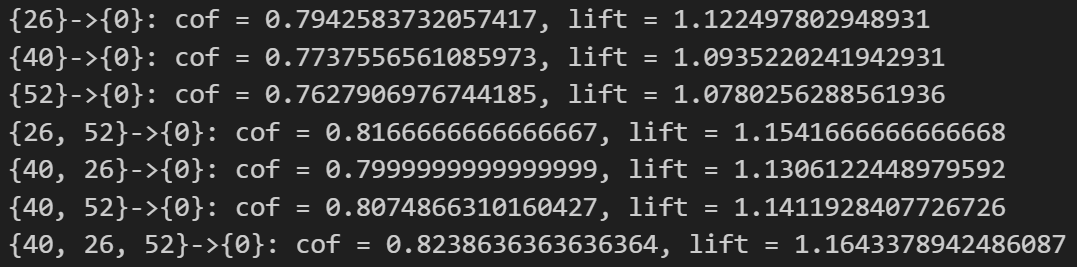
\includegraphics[height=3cm,width=12cm]{4.png}
	\end{figure}

   \subsection{Conclusion}	
   无结节帽、受侵淋巴结数目范围在0-2且未进行放疗与不复发强关联,我们可以认为出这部分患者不易复发乳腺癌。

\end{document}